
\chapter{Introduction}
\label{sec:orgae6eeaf}
\section{Motivation}
\label{sec:orgaf3be1e}

\section{Problem Statement}
\label{sec:org3eee55a}

\subsection{Motivation}
\label{sec:orga202d4f}
\emph{Can some device run a given algorithm?}

\emph{How the mapping process affect the circuit "probability of success"?}

\begin{figure}[htbp]
\centering
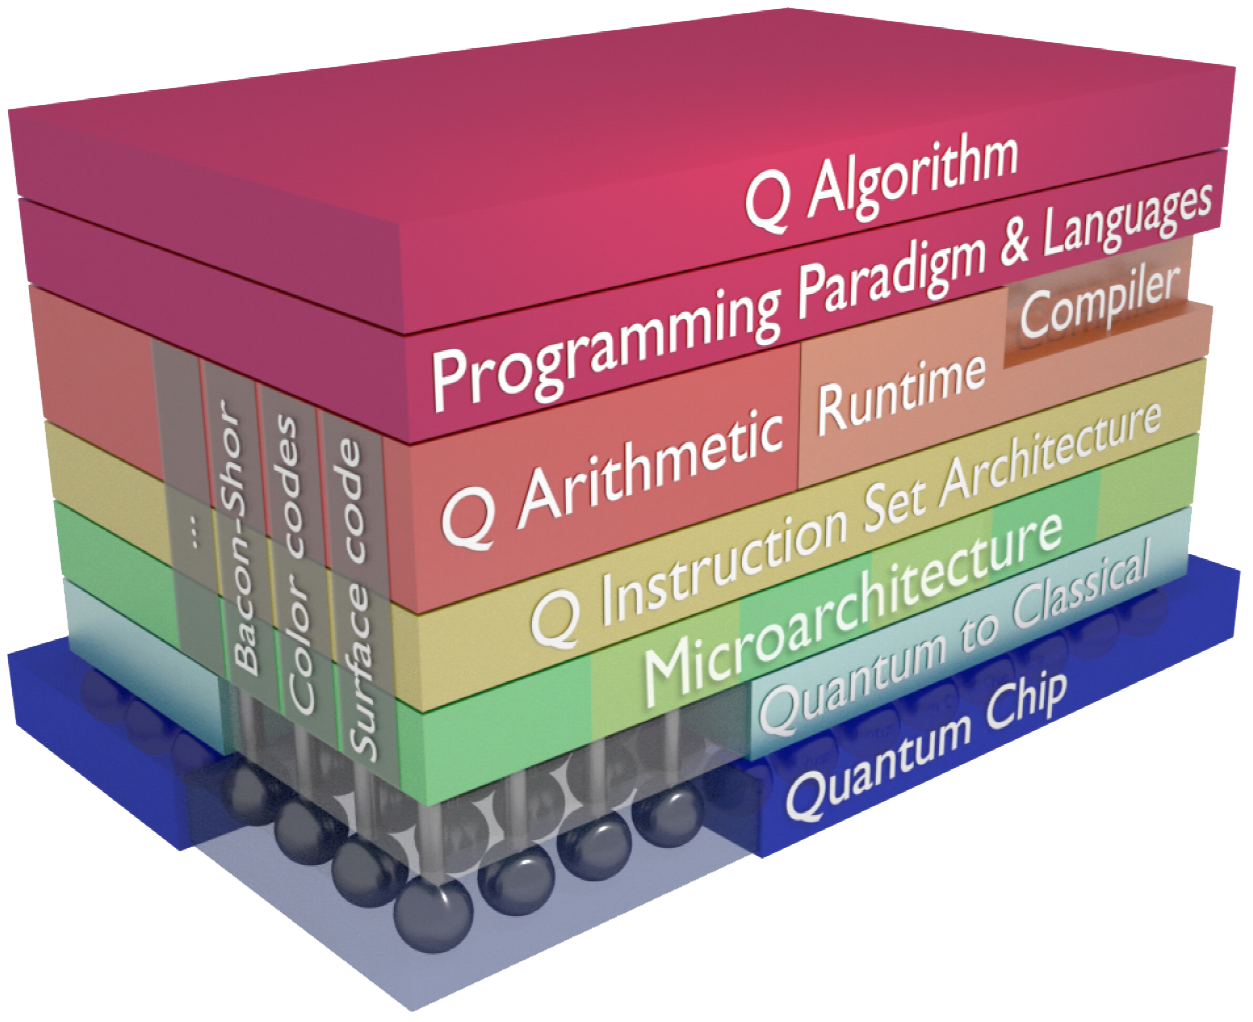
\includegraphics[width=0.7\textwidth]{figures/system_stack.png}
\caption{\label{fig:orgefabe52}
Full stack implementation}
\end{figure}

\subsection{Realization}
\label{sec:orgc159807}
The work is centered in:

\begin{itemize}
\item SC-7 and SC-17 chips
\item Physical level, without error correction
\item Two error models:
\begin{itemize}
\item Pauli Noise (QX simulator)
\item Complex empirical error model (quantumsim)
\end{itemize}
\end{itemize}

\section{Structure of the thesis}
\label{sec:orgb8ade80}
